\documentclass[11pt]{amsart}
\usepackage{geometry}                % See geometry.pdf to learn the layout options. There are lots.
\geometry{a4paper}                   % ... or a4paper or a5paper or ... 
%\geometry{landscape}                % Activate for for rotated page geometry
%\usepackage[parfill]{parskip}    % Activate to begin paragraphs with an empty line rather than an indent
\usepackage{graphicx}
\usepackage{amssymb, amsmath, amsthm}
\usepackage{natbib}
\usepackage{epstopdf}
\usepackage{enumerate}
\usepackage{textcomp}
\usepackage{mathrsfs }
\usepackage[section]{algorithm}
\usepackage{algorithmic}
\usepackage{tikz}
\usepackage{pgfplots}
\usepgfplotslibrary{patchplots}
%\usepackage{subfigure}
\usepackage{subcaption}

\usepackage{hyperref}
\usepackage{comment}
\usepackage{multirow}

%line suggested by my compiler (Fabian)
\pgfplotsset{compat=1.9}

% put figures at the end of the document, while I am writing is very annoying to have the figures in the middle of the text! 
% \usepackage[nomarkers,figuresonly]{endfloat}


\DeclareGraphicsRule{.tif}{png}{.png}{`convert #1 `dirname #1`/`basename #1 .tif`.png}

% \theoremstyle{theorem}
\newtheorem{theorem}{Theorem}[section]
\newtheorem{lemma}[theorem]{Lemma}
\newtheorem{proposition}[theorem]{Proposition}
\newtheorem{corollary}[theorem]{Corollary}
\newtheorem{point}[theorem]{}
\newtheorem{assumption}[theorem]{Assumption}


\theoremstyle{definition}
\newtheorem{definition}[theorem]{Definition}
\newtheorem{example}[theorem]{Example}
\newtheorem{notation}[theorem]{Notation}
\newtheorem{remark}[theorem]{Remark}
\newtheorem{condition}{Condition}

\newcommand{\F}{\operatorname{\mathcal{F}}}
\newcommand{\iF}{\operatorname{\mathcal{F}^{-1}}}

\newcommand{\Loperator}{\mathcal{L}}
%\newcommand{\R}{\mathbf{R}}
\newcommand{\Z}{\mathbf{Z}}

\newcommand{\dd}{\, \textrm{d}}
\newcommand{\e}{\textrm{exp}}
\newcommand{\fFrequency}{ f_{\omega_0}}
\newcommand{\fQuadrature}{ f_{\Delta}}

\newcommand{\I}{\mathbf{I}}

\newcommand{\ErrorFrequency}{\mathcal{E_F}}
\newcommand{\ErrorQuadrature}{\mathcal{E_Q}}
\newcommand{\Error}{\mathcal{E}}
\newcommand{\EF}{\ErrorFrequency}
\newcommand{\EQ}{\ErrorQuadrature}
\newcommand{\E}{\Error}
\newcommand{\est}{\overline {\mathcal{E}}}
\newcommand{\estFrequency}{\est_F}
\newcommand{\estQuadrature}{\est_Q}


\newcommand{\lx}{\mathcal{L}^{X}}
\newcommand{\ls}{\mathcal{L}^{S}}
\newcommand{\R}{\mathbb{R}}
\newcommand{\C}{\mathbb{C}}
\newcommand{\prob}[2]{\pi_{{#1,#2}}}
\newcommand{\lam}[1]{\lambda_#1}
\newcommand{\trials}[2]{\theta_{#1,#2}}
\newcommand{\damp}{\alpha}

\newcommand{\cgmyY}{Y}
\newcommand{\cgmyM}{\eta_+}
\newcommand{\cgmyG}{\eta_-}
\newcommand{\cgmyC}{K}

\newcommand{\cgmyexp}{\cgmyY}

\newcommand{\fa}{f_{\damp}}
\newcommand{\fadisc}[1]{f_{\damp, #1}}
\newcommand{\fdisc}[1]{f_{#1}}
\newcommand{\ga}{g_{\damp}}
\newcommand{\ha}{h_{\damp}}
\newcommand{\ft}[1]{\hat{#1}}
\newcommand{\kft}[1]{\tilde{#1}}
\newcommand{\ift}[1]{\iF\left[#1\right]}
\newcommand{\Lnorm}{\textrm{L}}
\newcommand{\real}[1]{\mathrm{Re}\left[#1\right]}
\newcommand{\im}[1]{\mathrm{Im}\left[#1\right]}
\newcommand{\step}{\Delta\omega}
\newcommand{\strip}[1]{A_{#1}}
\newcommand{\pureJumpProcessConstant}{C(\nu)}
\newcommand{\ffreq}[1]{\nu_{#1}}


\newcommand{\charExp}[1]{\Psi \parent{{#1}}}
\newcommand{\charFun}[2]{\varphi_{#1} \parent{{#2}}}

\newcommand{\cutoff}{\omega_{\mathrm{\max}}}
\newcommand{\strike}{k}

\newcommand{\pprob}[1]{}

\newcommand{\fnka}{f_{\damp}^{N,\cutoff}}
\newcommand{\ftnka}{\tilde f_{\damp}^{N,\cutoff}}

\newcommand{\pnka}{\Pi_{\damp}^{N,\cutoff}}

\newcommand{\fft}[2]{\mathrm{FFT}_{{#1}} \parent{{#2} }}
\newcommand{\tol}{\epsilon_{\mathrm T}}

\newcommand{\cutoffFrequency}{\omega_{\textrm{max}}}

\newcommand{\uremark}[2]{\underbrace{{#1}}_{{#2}}}

% Juho macros
\newcommand{\partder}[2]{\frac{\partial #1}{\partial #2}}
\newcommand{\der}[1]{\partial_{ #1}}
\newcommand{\ket}[1]{\left | {#1} \right \rangle }
\newcommand{\refstate}[0]{\textbf{0}}
\newcommand{\vacket}[0]{\ket{\refstate}}
\newcommand{\vacbra}[0]{\bra{\refstate}}
\newcommand{\bra}[1]{\left \langle {#1} \right | }
\newcommand{\ketbra}[1]{\ket{#1} \bra{#1}}
\newcommand{\innerprod}[2]{\left \langle {{#1} | {#2}} \right \rangle}
\newcommand{\uket}[0]{\ket{\uparrow}}
\newcommand{\dket}[0]{\ket{\downarrow}}
\newcommand{\ubra}[0]{\bra{\uparrow}}
\newcommand{\dbra}[0]{\bra{\downarrow}}
\newcommand{\hadj}[1]{{#1}^{\dagger}}
\newcommand{\conj}[1]{{#1}^{\ast}}
\newcommand{\cosine}[1]{\mathrm{cos}\left ( {#1}\right )}
\newcommand{\sine}[1]{\mathrm{sin}\left ( {#1}\right )}
\newcommand{\cosinep}[2]{\mathrm{cos}^{#2}\left ( {#1}\right )}
\newcommand{\sinep}[2]{\mathrm{sin}^{#2}\left ( {#1}\right )}
\newcommand{\expf}[1]{\mathrm{exp}\left ( {#1}\right )}
\newcommand{\expfs}[1]{e^{#1}}
\newcommand{\determinant}[1]{\mathrm{det}\left ( {#1}\right )}
\newcommand{\trace}[1]{\mathrm{Tr}\left ( {#1}\right )}
\newcommand{\parent}[1]{\left( {#1} \right)}
\newcommand{\aver}[1]{ \left\langle  {#1}  \right\rangle }
\newcommand{\absval}[1]{\left| {#1} \right|}
\newcommand{\sset}[1]{\left\lbrace {#1} \right\rbrace }
\newcommand{\iden}[1]{\mathbf{1}_{#1}}
\newcommand{\ssum}[2]{\displaystyle\sum\limits_{#1}^{#2}}
\newcommand{\pprod}[2]{\displaystyle\prod\limits_{#1}^{#2}}
\newcommand{\commut}[2]{\left[ {#1} , {#2} \right]}
\newcommand{\acommut}[2]{\left\lbrace  {#1} , {#2} \right\rbrace }
\newcommand{\spann}[1]{\mathrm{span} \parent{{#1}}}
\newcommand{\ttrace}[2]{\mathrm{Tr}_{#1} \parent{#2}}
\newcommand{\logt}[1]{\mathrm{log_2} \parent{{#1}}}
\newcommand{\hilbert}[1]{\mathcal{H}_{{#1}}}
\newcommand{\genus}{g}
\newcommand{\gsfun}[0]{\eta_{GS}}
\newcommand{\vvec}[1]{\textbf{{#1}}}
\newcommand{\kk}[0]{\vvec{k}}
\newcommand{\tsection}[1]{\newpage \section{{#1}}}
\newcommand{\grad}[0]{\nabla}
\newcommand{\divv}[0]{\nabla \dot}
\newcommand{\curl}[0]{\nabla \times}
\newcommand{\vvar}[1]{\mathrm{var} \parent{{#1}}}
\newcommand{\bigo}[1]{\mathcal O \parent{{#1}}}
\newcommand{\smallo}[1]{ o \parent{{#1}}}
\def\d{\textrm{d}}

\newcommand{\cost}[1]{C_{\mathrm{#1}}}

\newcommand{\qt}[0]{\tilde q}
%\newcommand{\e}[1]{\times 10^{#1}}
\newcommand{\supremum}[1]{\mathop{\mathrm{sup}}_{{#1}}}
\newcommand{\nnorm}[2]{\absval{\absval{{#1}}}_{#2}}
\newcommand{\problem}[1]{\newpage \section*{{#1}}}
\newcommand{\hittime}[0]{\sigma_{\bar{\mathcal E}}}
\newcommand{\probb}[1]{\mathrm{P} \parent{{#1}}}
\newcommand{\expp}[1]{\mathrm{E} \parent{{#1}}}

\newcommand{\kaustaddress}[0]{King Abdullah University of Science and Technology, Thuwal, Kingdom of Saudi Arabia}
\newcommand{\indicatorfun}[3]{\mathbf{1}_{[{#1},{#2}]} \parent{{#3}}}
\newcommand{\indicator}{\mathbf{1}}
\newcommand{\binaryg}[1]{g_{\mathrm{bin}} \parent{#1}}
\newcommand{\binaryf}[1]{f_{\mathrm{bin}} \parent{#1}}
\newcommand{\fbinaryf}[1]{\hat{f}_{\mathrm{bin}} \parent{#1}}

\newcommand{\callg}[1]{g_{\mathrm{call}} \parent{#1}}
\newcommand{\fcallg}[1]{\hat{g}_{\mathrm{call}} \parent{#1}}
\newcommand{\fcallga}[1]{\hat{g}_{\mathrm{call}, \damp} \parent{#1}}
\newcommand{\fputga}[1]{\hat{g}_{\mathrm{put}, \damp} \parent{#1}}
\newcommand{\fcallf}[1]{\hat{f}_{\mathrm{call}} \parent{#1}}
\newcommand{\fcallfa}[1]{\hat{f}_{\mathrm{call}, \damp} \parent{#1}}


\newcommand{\evaldiff}[3]{{\left [ {#1} \right ]}_{#2}^{#3}} 

\newcommand{\vga}{a}
\newcommand{\vgb}{b}

\newcommand{\vgpoly}[1]{w  \parent{#1}}
\newcommand{\vgaux}{q}

\newcommand{\imo}{y}
\newcommand{\reo}{x}
\newcommand{\abex}{\rho}

%%% for the merton case
\newcommand{\sj}{\sigma_{\mathrm{jump}}}
\newcommand{\rj}{r_{\mathrm{jump}}}


%% I always forget the correct spelling
\newcommand{\levy}{L\'evy }
\newcommand{\levynospace}{L\'evy}
%%

\newcommand{\rz}{\R \setminus \sset{0}}

\newcommand{\linf}[1]{L^\infty_{#1}}
\newcommand{\norminf}[2]{\left\|#1\right\|_{\linf{#2}}}
\newcommand{\cl}{C \parent{\lambda}}

\pgfmathdeclarefunction{lg10}{1}{%
    \pgfmathparse{ln(#1)/ln(10)}%
}


\title[MIMC and MLMC HJM]{Multi-Index and Multi-Level Monte Carlo Evaluation of HJM Models}
\author{Juho H\"app\"ol\"a}
\address{\kaustaddress}
\email{juho.happola@iki.fi}


\date{\today}    
                                    % Activate to display a given date or no date
\begin{document}


\begin{abstract}
Notes of MIMC and MLMC evaluation of HJM models.
\end{abstract}

\maketitle
%\tableofcontents


\section{HJM model in Fourier space}

Let us focus on the following HJM type SDE:
\begin{align}
d f \parent{t,\tau} &= \alpha \parent{t,\tau} dt + \beta \parent{t,\tau} d \overline W \parent t \\
f \parent{0,\tau} &= f_0 \parent \tau ,
\end{align}
with the diffusion term given as the infinite-dimensional extension of
eq. (1.1) in \cite{bjork2013monte}:
\begin{align}
%\beta \parent{t, \tau} d \overline W \parent t = \ssum{k=0}{\infty} c_n \parent{\sin %\parent{\ffreq{k} \tau} + \cos \parent{\ffreq{k} \tau} dW_n \parent t , 
\beta \parent{t, \tau} d \overline W \parent t = \ssum{k=0}{\infty}
c_n \parent{ \sin \parent{\ffreq k \tau} + \cos \parent{\ffreq k \tau} }
\end{align}
with $W_n$ independent Brownian motions and
\begin{align*}
\ffreq k \equiv \frac{k \pi }{L}
\end{align*}
with $L>>1$. This gives the following Fourier decomposition for the covariance
of increments:
\begin{align}
&\expp{ \beta \parent{t, \tau_1} d \overline W \parent t \beta \parent{t, \tau_2} d \overline W \parent t}
\\
= & \ssum{k=0}{\infty} c_k^2 \parent{ \cos \parent{\ffreq k \parent{\tau_1-\tau_2}}}
\end{align}

To keep the exponential HJM model risk neutral, we fix the drift of the equation as
\begin{align*}
\alpha \parent{t, \tau} 
=&
c_0^2 \parent{\tau-t}
\\
&+
\ssum{k=1}{\infty }
\frac{c_k^2}{k}
\sin \parent{\ffreq k \tau } \parent{\cos \parent{\ffreq q t} -  \sin \parent{\ffreq k t}}
\\
&+
\ssum{k=1}{\infty }
\frac{c_k^2}{k}
\cos \parent{ \ffreq k \tau } \parent{\cos \parent{\ffreq k t} -  \sin \parent{\ffreq k t}}
\\
&+
\ssum{n=1}{\infty }
\frac{c_n^2}{n}
\cos \parent{2 \ffreq k \tau }.
\end{align*}

The solution to the SDE can be written as
\begin{align*}
f \parent{t,\tau} - f_0 \parent \tau
= \tilde f \parent{t,\tau}
+ \ssum{n=1}{N} b_n \parent t \cos \parent{\frac{n \pi \tau}{L}} + a_n \parent t \sin \parent{\frac{n \pi \tau}{L}},
\end{align*}
with
\begin{align}
\tilde f \parent{t,\tau} =& c_0^2 t \parent{\tau-\frac{t}{2}},
\\
a_k \parent{t} = b_k \parent t =& \frac{c_k^2}{\ffreq k^2}\parent{\cos \parent{\ffreq k t} + \sin \parent{\ffreq k t}-1 } - \frac{\mathbf{1}_{\frac{k}{2} \in \mathbb Z_+}  c_j^2  t}{\ffreq k}  + c_k W_k \parent{t} .
\end{align}

The solution above lends itself to approximate solutions to the quantity of interest.
First, the discount factor can be approximated as:
\begin{align*}
&\int_0^{T} f \parent{s,s} ds
\\
\approx& \Delta t \ssum{n=1}{N_t} \parent{ f_0 \parent{t_n} + \tilde f \parent{t_n, t_n} +
\ssum{k=1}{N_f}
b_k \parent {t_n} \cos \parent{ \ffreq k t_n} + a_k \parent {t_n} \sin \parent{\ffreq k t_n}
}
\\
=& F_{N_t,N_f}
,
\end{align*}
with $t_n = \frac{nT}{N_t}$.
This approximation gives the following approximation error
in $N_f$.

The natural next step is, of coures, estimating the error in approximating the
integral by $F_{N_t,N_f}$. Firstly, there is the case of the frequency cutoff:
\begin{align*}
&\expp{ \parent{\int_0^T f \parent{s,s} ds - \lim_{N_t \rightarrow \infty} F_{N_t,N_f}}^2}
\\
=& \expp{\int_0^T \ssum{k=N_f+1}{\infty} \parent{b_k \parent{t_n} \cos \parent{\ffreq k t_n} + a_k \parent{t_n} \sin \parent{\ffreq k t_n}} ds}
\\
\approx &
\expp{\parent{\int_0^T \ssum{k=N_f+1}{\infty} c_k W_k \parent{t} \parent{\sin \parent{\ffreq k t} + \cos \parent{\ffreq k t} }}^2}
\\
= &
\expp{\parent{ \ssum{k=N_f+1}{\infty} \int_0^T c_k W_k \parent{t} \parent{\sin \parent{\ffreq k t} + \cos \parent{\ffreq k t} } ds}^2}
\\
= & \bigo{\ssum{k=N_f+1}{\infty} \parent{\frac{c_k}{k}}^2}.
\end{align*}
A bound for the bias error can be obtained using Jensen's inequality. Setting as a test
case the temporal correlation structure as
$
\rho \parent{\tau_1, \tau_2} \propto \expf{ - \kappa \absval{\tau_1-\tau_2}}
$
it follows that $c^2_k =\frac{\kappa}{L} \frac{\parent{-1}^k\parent{1-\expf{-\absval{\kappa L}}}}{\kappa^2 + \parent{\ffreq k}^2}$. Using this as an example, we plot the empirical strong and weak convergence rates in figure \ref{fig:rateFig1}.

\begin{figure}
    \centering
    \begin{subfigure}[b]{0.4\textwidth}
        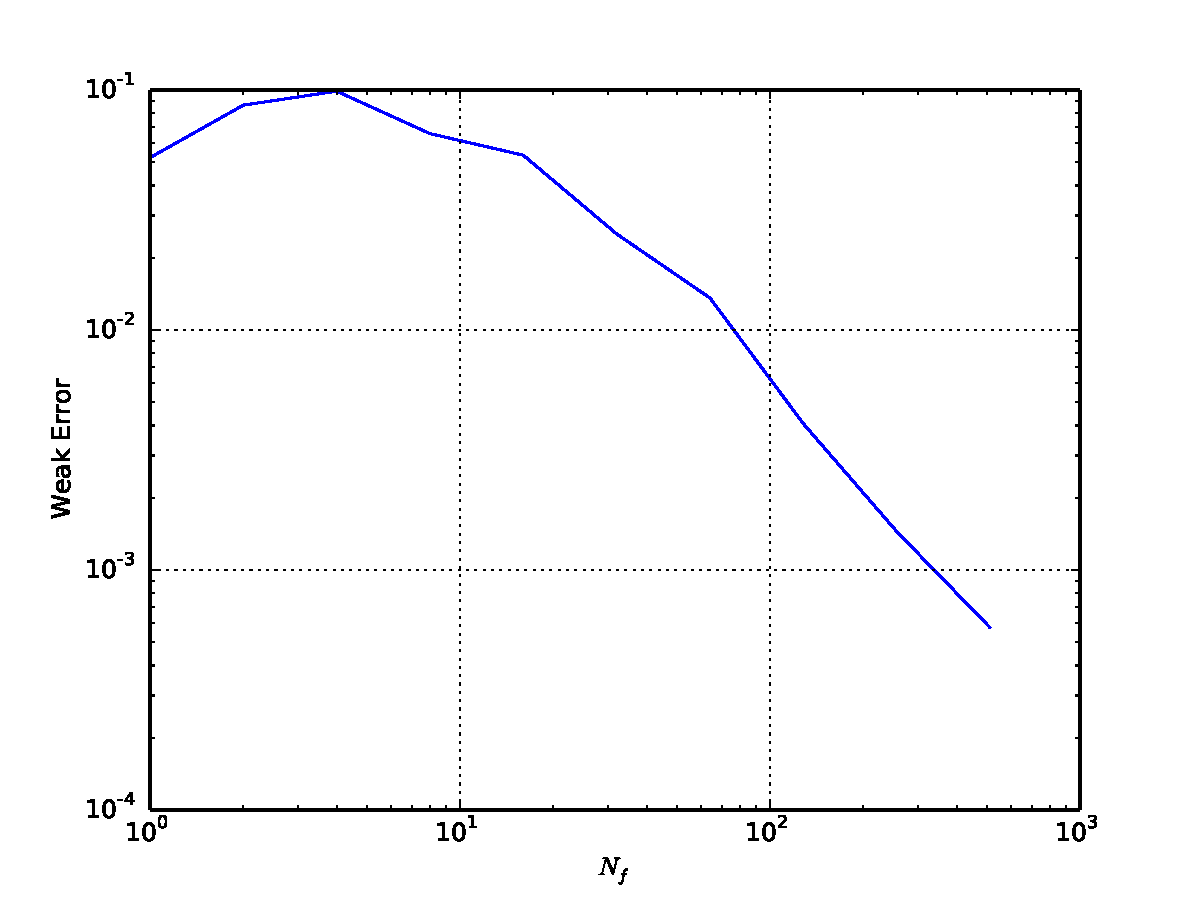
\includegraphics[width=\textwidth]{weakerr1.pdf}
        %\caption{A gull}
    \end{subfigure}
    ~ %add desired spacing between images, e. g. ~, \quad, \qquad, \hfill etc. 
      %(or a blank line to force the subfigure onto a new line)
    \begin{subfigure}[b]{0.4\textwidth}
        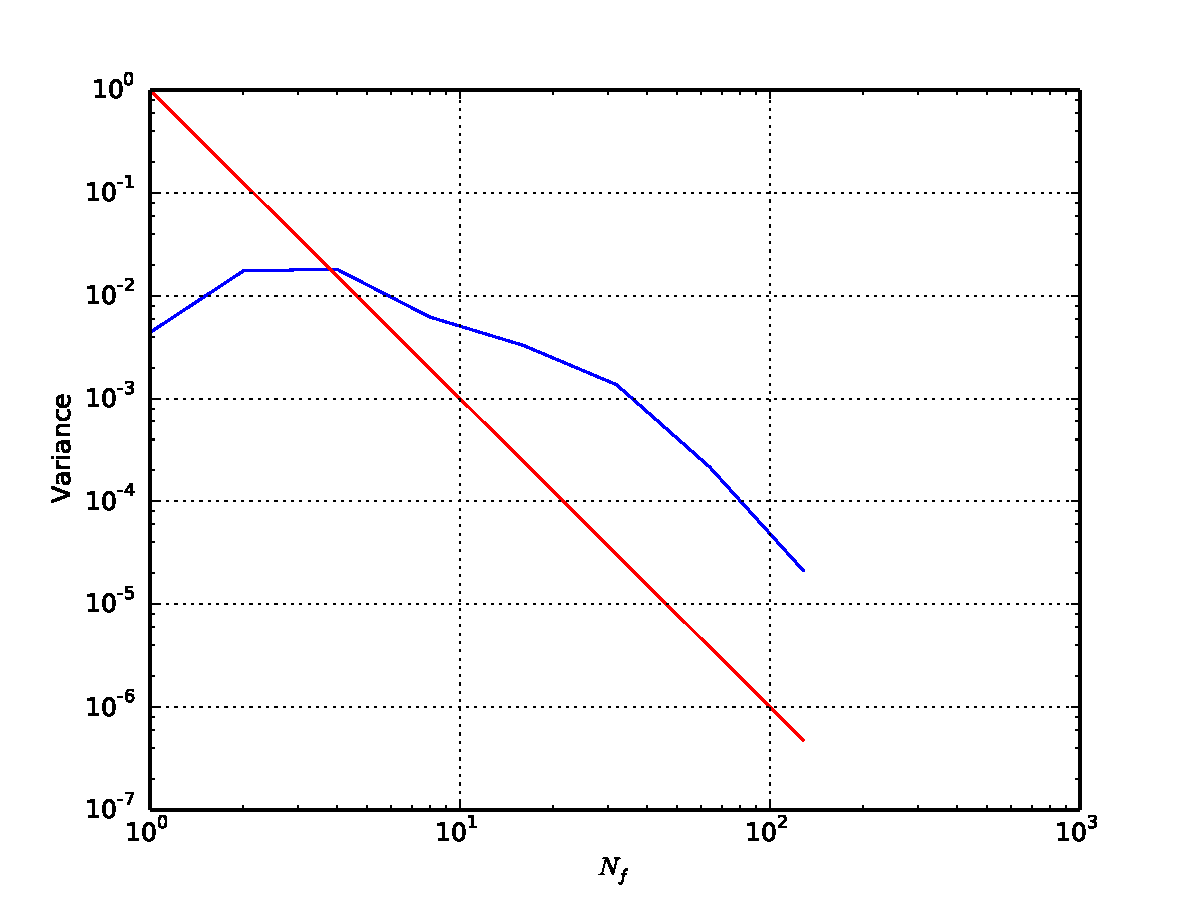
\includegraphics[width=\textwidth]{strongerr1.pdf}
        %\caption{A tiger}
    \end{subfigure}
    \caption{\label{fig:rateFig1} Bias (left) and variance (right) error
    $\nnorm{F_{513,2N_f} - F_{513,N_f}}{}$ along with $N_f^{-\frac{3}{2}}$ and
    	$N_f^{3}$ reference lines in red.}
\end{figure}

As for the time discretisation error, we are concerned with a rectangle quadrature
error, giving us weak and strong error rate of $1$ and $2$ respectively. Empirical
test of these rates is presented in figure \ref{img:rateFig3}.

\begin{figure}
    \centering
    \begin{subfigure}[b]{0.4\textwidth}
        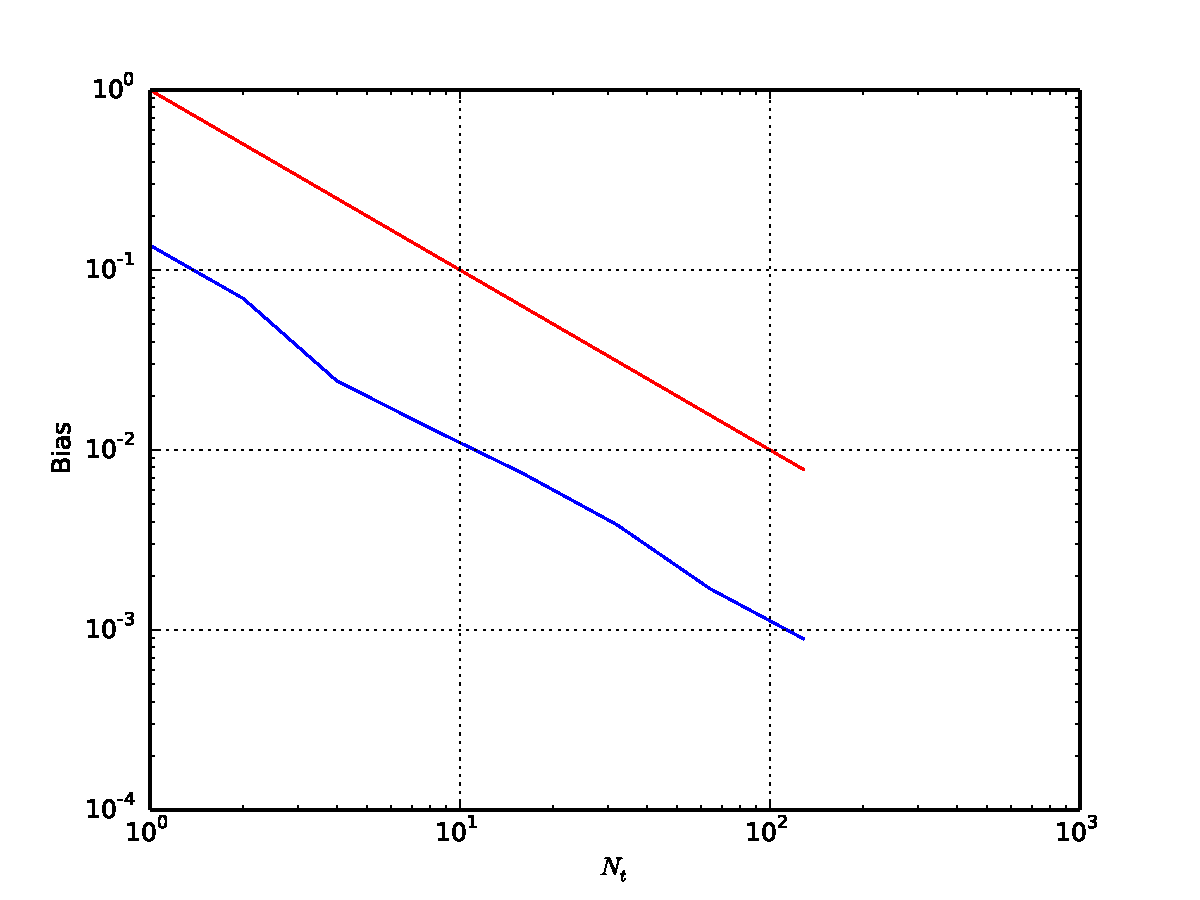
\includegraphics[width=\textwidth]{weakerr3.pdf}
        %\caption{A gull}
    \end{subfigure}
    ~ %add desired spacing between images, e. g. ~, \quad, \qquad, \hfill etc. 
      %(or a blank line to force the subfigure onto a new line)
    \begin{subfigure}[b]{0.4\textwidth}
        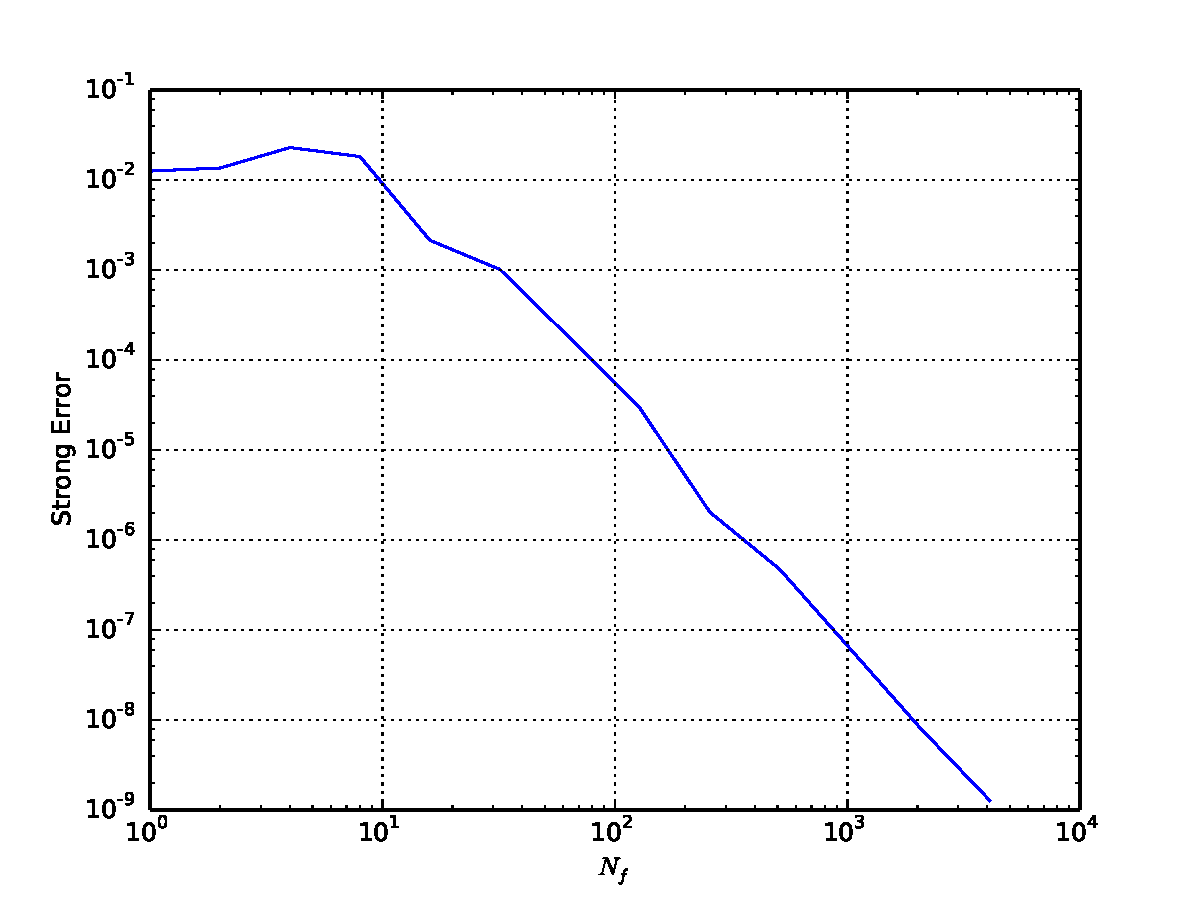
\includegraphics[width=\textwidth]{strongerr3.pdf}
        %\caption{A tiger}
    \end{subfigure}
    \caption{\label{img:rateFig3} Bias (left) and variance (right) error
    for the temporal discretisation
    $\nnorm{F_{2N_t-1,16}-F_{N_t,16}}{}$
    along with $N_t^{-1}$ and $N_t^{-2}$ reference lines in red.}
\end{figure}

Similarly, one may estimate the underlying part of the 
payoff functional
\begin{align*}
&\int_{\tau_1}^{\tau_2}
f \parent{T,\tau} d\tau 
\\
\approx & \int_{\tau_1}^{\tau_2}
f_0 \parent \tau + \tilde f \parent{t_n, t_n} +
\ssum{k=1}{N_f}
b_k \parent T \cos \parent{\ffreq k \tau} + a_k \parent {T} \sin \parent{\ffreq k \tau}
d \tau.
\\
= & \int_{\tau_1}^{\tau_2}
f_0 \parent \tau  + \frac{c_0 T}{2} \parent{\tau_2^2 - \tau_2 +\tau_1 - \tau_1^2} d \tau
\\
&+
\ssum{k=1}{N_f} 
\frac{b_k \parent T}{\ffreq k } 
\parent{\sin \parent{\ffreq k \tau_2}  - \sin \parent{\ffreq k \tau_1} }
\\
&-
\ssum{k=1}{N_f} 
\frac{a_k \parent T}{\ffreq k} 
\parent{\cos \parent{\ffreq k \tau_2}  - \cos \parent{\ffreq k \tau_1} }
\\
=& \Psi_{N_f} .
\end{align*}
This approximation has its own approximation error with respect to $N_f$:
\begin{align*}
&\expp{\parent{\int_{\tau_1}^{\tau_2} f \parent{T,\tau} d \tau - \Psi_{N_f}}^2}
\\
=& \expp{\parent{\ssum{k=N_f+1}{\infty} \frac{b_k \parent T}{\ffreq k } 
\parent{\sin \parent{\ffreq k \tau_2}  - \sin \parent{\ffreq k \tau_1} } - \frac{a_k \parent T}{\ffreq k} 
\parent{\cos \parent{\ffreq k \tau_2}  - \cos \parent{\ffreq k \tau_1} }  }^2}
\\
= & \bigo{\ssum{k = N_f+1}{\infty} \frac{c_k^2}{\ffreq k^2}}.
\end{align*}
Using the exponentially decaying covariance function, we expect order $3$ strong convergence
and, using Jensen's inequality, we may bound the weak error to order $\frac{3}{2}$. Accompanying numerical rates are presentend in figure \ref{img:rateFig2}.

\begin{figure}
    \centering
    \begin{subfigure}[b]{0.4\textwidth}
        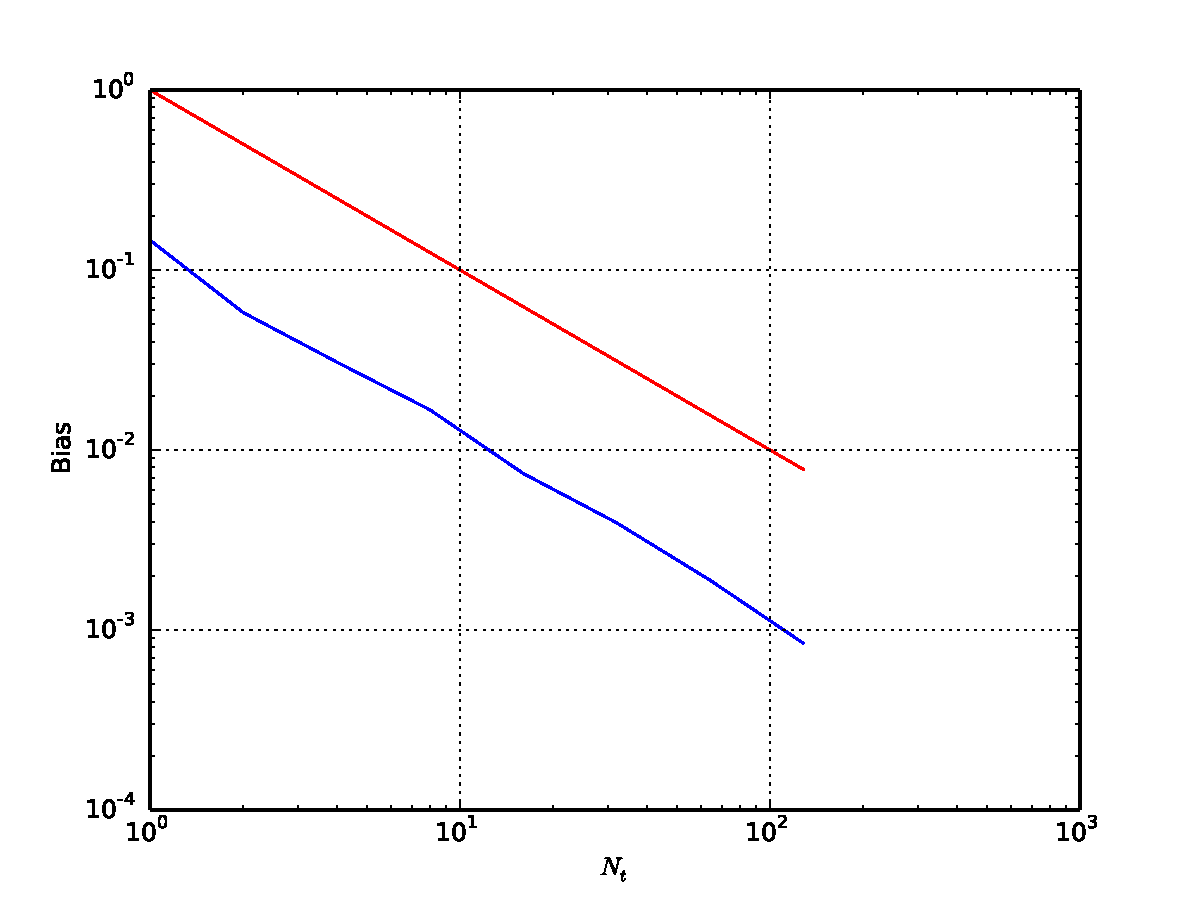
\includegraphics[width=\textwidth]{weakerr2.pdf}
        %\caption{A gull}
    \end{subfigure}
    ~ %add desired spacing between images, e. g. ~, \quad, \qquad, \hfill etc. 
      %(or a blank line to force the subfigure onto a new line)
    \begin{subfigure}[b]{0.4\textwidth}
        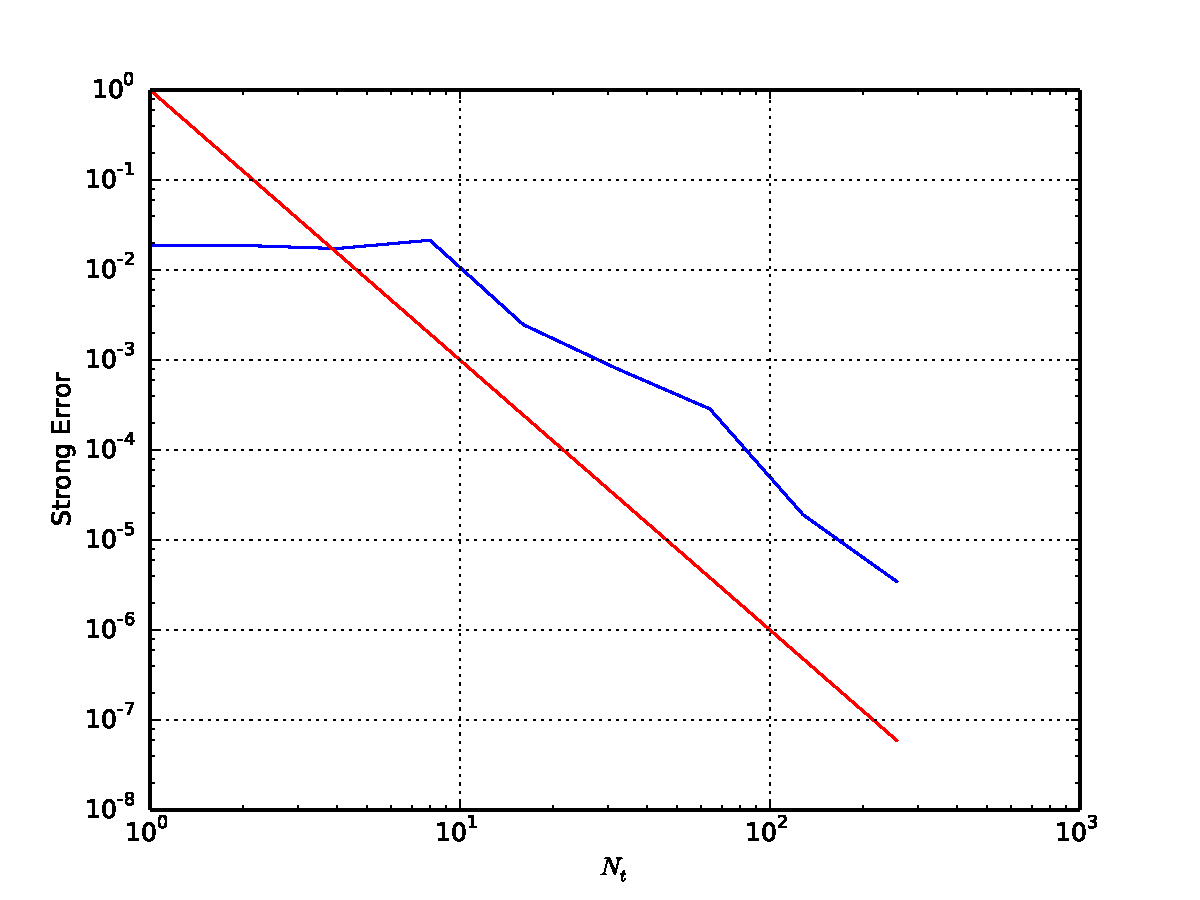
\includegraphics[width=\textwidth]{strongerr2.pdf}
        %\caption{A tiger}
    \end{subfigure}
    \caption{\label{img:rateFig2} Bias (left) and variance (right) error
    for frequency cutoff
    $\nnorm{\Psi_{2N_f}-\Psi_{N_f}}{}$ together with the $N_f^{-\frac{3}{2}}$ and
    $N_f^{-3}$ reference lines in red.}
\end{figure}

Overall, we may approximate a future price of a zero-coupon bond as
\begin{align*}
\mathcal G \parent f =&
\expp{\expf{-\int_0^{t_{T}} f \parent{s,s} ds}\expf{-\int_{\tau_1}^{\tau_2} f \parent{T,\tau} d\tau}}
\\
\approx&
\underbrace{\expp{\expf{-
F_{N_t,N_f}-
\Psi_{N_f} }}}_{\overline G_{N_t,N_f}}.
\end{align*}
Continuing the case of exponential covariance structure where $c_k \sim \bigo{k^{-2}}$,
we expect, based on the above computations, to observe the following rate
\begin{align*}
\expp{ \parent{\mathcal G - \overline G_{N_t,N_f}}^2} = \bigo{N_f^{-3} N_t^{-2}}.
\end{align*} 
To complement the component-wise plots in figures \ref{fig:rateFig1}, \ref{img:rateFig2} and
\ref{img:rateFig3}, we plot the overall approximation of $\mathcal G$ with $\overline G_{N_t,N_f}$
in figure \ref{img:rateFig4}.

\begin{figure}
    \centering
    \begin{subfigure}[b]{0.4\textwidth}
        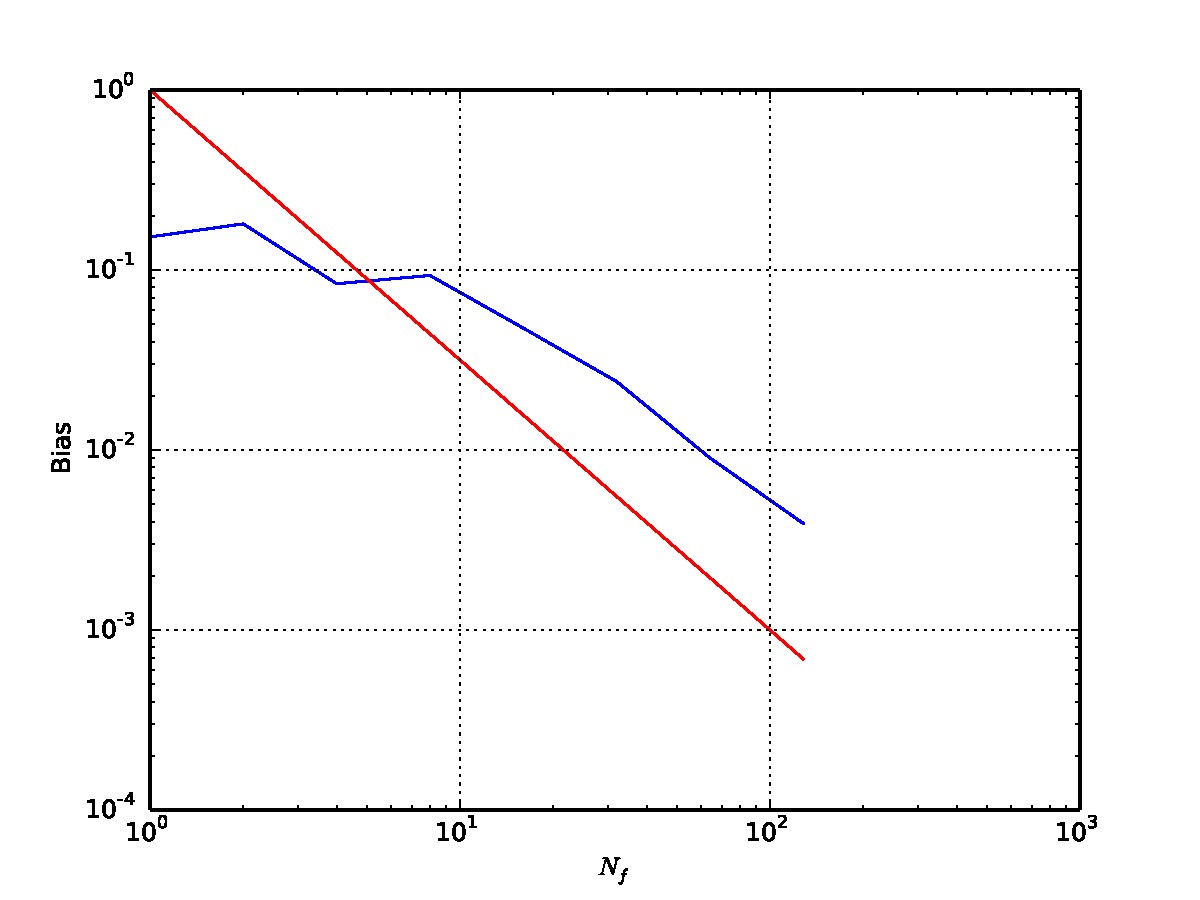
\includegraphics[width=\textwidth]{weakerr4.pdf}
        %\caption{A gull}
    \end{subfigure}
    ~ %add desired spacing between images, e. g. ~, \quad, \qquad, \hfill etc. 
      %(or a blank line to force the subfigure onto a new line)
    \begin{subfigure}[b]{0.4\textwidth}
        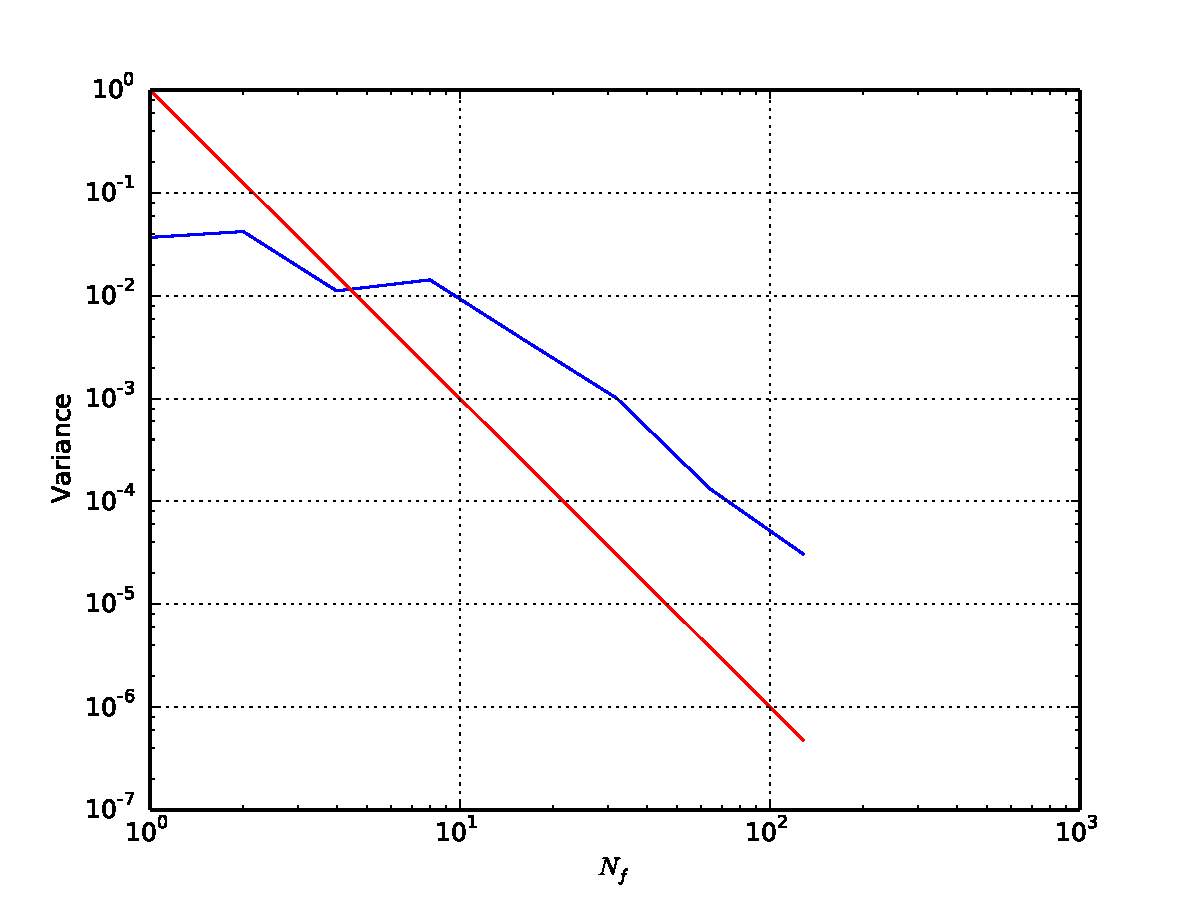
\includegraphics[width=\textwidth]{strongerr4.pdf}
        %\caption{A tiger}
    \end{subfigure}
    \\
        \begin{subfigure}[b]{0.4\textwidth}
        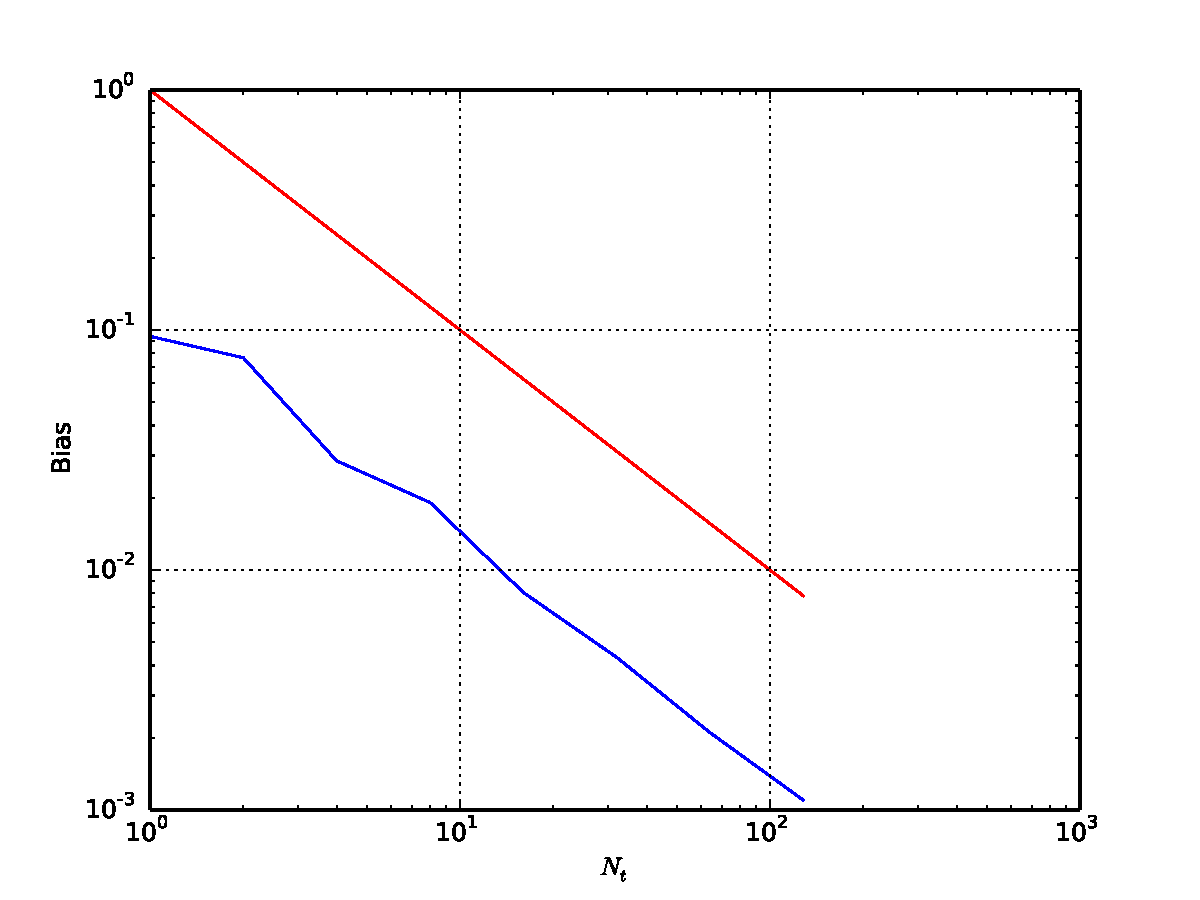
\includegraphics[width=\textwidth]{weakerr5.pdf}
        %\caption{A gull}
    \end{subfigure}
    ~ %add desired spacing between images, e. g. ~, \quad, \qquad, \hfill etc. 
      %(or a blank line to force the subfigure onto a new line)
    \begin{subfigure}[b]{0.4\textwidth}
        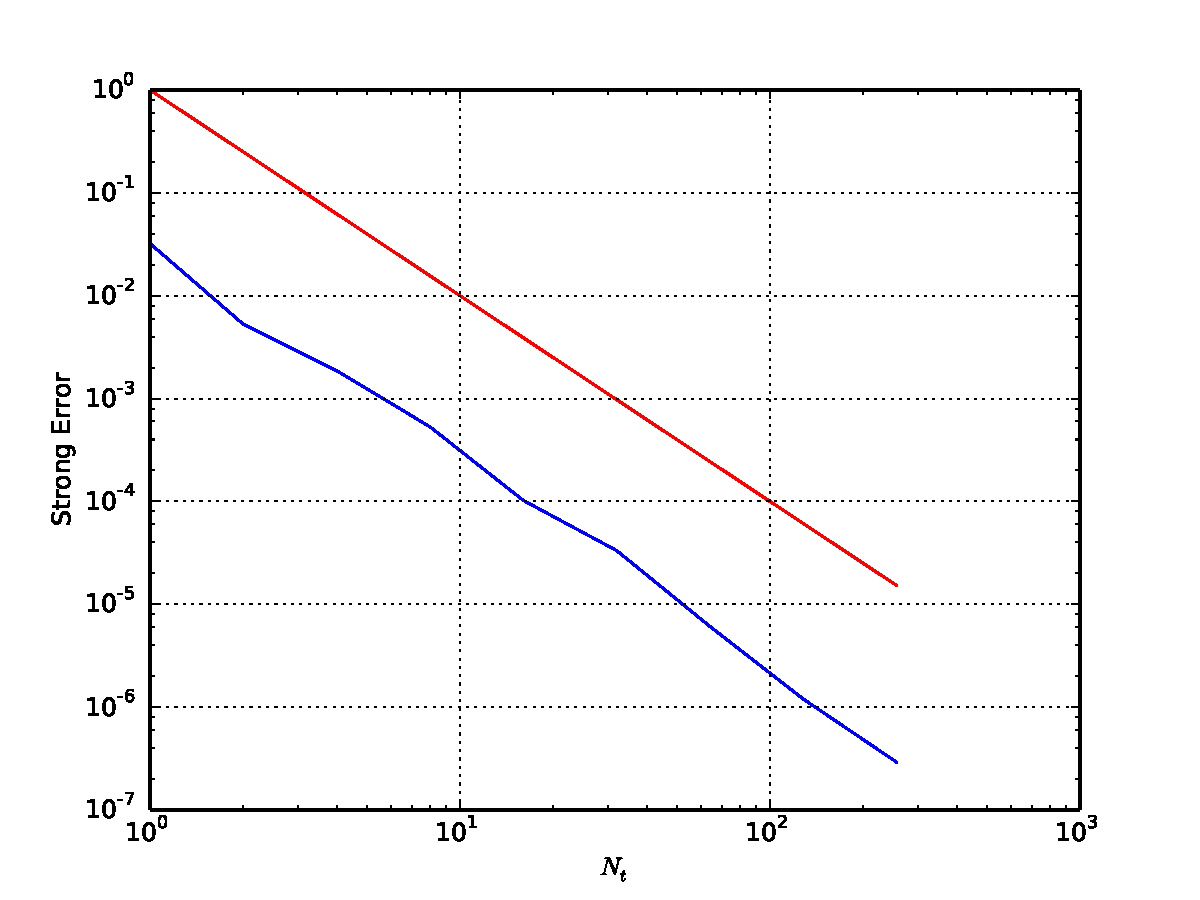
\includegraphics[width=\textwidth]{strongerr5.pdf}
        %\caption{A tiger}
    \end{subfigure}
    \caption{\label{img:rateFig4} Above: Bias (left) and variance (right) error
    for the cutoff
    $\nnorm{\overline G_{65,2N_f}-\overline G_{65,N_f}}{}$,
    along with the $N_f^{-\frac{3}{2}}$ and $N_f^{3}$ reference lines (red).
    Below: Bias (left) and variance (right) error for the temporal discretisation
    $\nnorm{\overline G_{2N_t-1,16} - \overline G_{N_t,16}}{}$ with the 
    $N_t^{-1}$ and $N_t^{-2}$ reference lines for the bias and variance error,
    respectively (red).}
\end{figure}

Setting $\ell = \parent{\ell_1 , \ell_2}$, we may define a Monte
Carlo estimator using $m$ independent realisations of $\overline G_{N_t,N_f}$:
\begin{align}
\mathcal A_{\ell_1, \ell_2} 
\equiv
\ssum{m=1}{M}
\frac{\overline G_{2^{\ell_1}+1,2^{\ell_2}} \parent m}{M}.
\end{align}

Similarly, we may extend the above to a MLMC estimator as
\begin{align*}
\mathcal{A}_{ML} =& \ssum{m=0}{M_0} \frac{\overline G_{2 C_1 ,C_2 } \parent m}{M_0}
\\
&+
\ssum{\ell_1=1}{L}
\ssum{m=0}{M_{\ell_1}} \frac{\parent{ \overline GF_{C_1 2^{\ell_1}+1,C_2 2^{\ell_1}} - \overline G_{C_1 2^{\ell_1-1}+1,C_2 2^{\ell_1-1}} } \parent m }{M_{\ell_1}},
\\
\equiv& \ssum{\ell_1=0}{L} \ssum{m=0}{M_{\ell_1}} \frac{\Delta_{\ell_1} \parent m}{M_{\ell_1}}
\end{align*}
and, into a MIMC estimator through defining the appropriate two-dimensional difference operators $\Delta_{\ell_1,\ell_2}$ and a downward-closed index-set $L_K=\sset{\parent{\ell_1,\ell_2}\in \mathbb Z_+^2: I \parent{\ell_1,\ell_2}<K}$:
\begin{align*}
\mathcal A_{MI} =& \ssum{\ell \in L_K}{} \ssum{m=1}{M_{\ell}} \frac{\Delta_{\ell_1,\ell_2} \parent m}{M_\ell}
\\
\Delta_{\ell_1,\ell_2}
\equiv&
\overline G_{C_1 2^{\ell_1}+1,C_2 2^{\ell_2}} - \mathbf{1}_{\ell_1>1} \overline G_{C_1 2^{\ell_1-1}+1,C_2 2^{\ell_2-1}} 
\\
& -\mathbf{1}_{\ell_2>1} \overline G_{C_1 2^{\ell_1-1}+1,C_2 2^{\ell_2}} 
+ \mathbf{1}_{\ell_1,\ell_2>1} \overline G_{C_1 2^{\ell_1-1}+1,C_2 2^{\ell_2-1}} .
\end{align*}


\bibliographystyle{agsm}
\bibliography{references}

\appendix




\end{document}


